\documentclass[final]{beamer}

% ====================
% Packages
% ====================

\usepackage[T1]{fontenc}
\usepackage[utf8]{inputenc}
\usepackage{lmodern}
\usepackage[size=custom,width=120,height=72,scale=1.0]{beamerposter}
\usetheme{gemini}
\usecolortheme{UA}
\usepackage{graphicx}
\usepackage{booktabs}
\usepackage{doi}
\usepackage[numbers]{natbib}
\usepackage[patch=none]{microtype}
\usepackage{tikz}
\usepackage{pgfplots}
\pgfplotsset{compat=1.18}
\usepackage{anyfontsize}

\pdfstringdefDisableCommands{%
\def\translate#1{#1}%
}

% ====================
% Lengths
% ====================

% If you have N columns, choose \sepwidth and \colwidth such that
% (N+1)*\sepwidth + N*\colwidth = \paperwidth
\newlength{\sepwidth}
\newlength{\colwidth}
\setlength{\sepwidth}{0.025\paperwidth}
\setlength{\colwidth}{0.3\paperwidth}

\newcommand{\separatorcolumn}{\begin{column}{\sepwidth}\end{column}}

% ====================
% Title
% ====================

%\makeatletter
%\def\title#1{\gdef\@title{\scalebox{\TP@titletextscale}{%
%\begin{minipage}[t]{\linewidth}
%\centering
%#1
%\title{Second order molecular properties from the random phase approximation (RPA)}
%\author{Sree Ganesh Balasubramani, Vamsee K. Voora, Filipp Furche}
%\institute{Department of Chemistry, University of California, Irvine, USA}
%\par
%\vspace{0.5em}
%\end{minipage}%
%}}}
%\makeatother
\title{Transition path sampling analysis}
\author{Sree Ganesh Balasubramani, Steven Schwartz}
\institute{Department of Chemistry and Biochemistry, University of Arizona}
%\titlegraphic{\includegraphics[scale=0.52]{uci.jpg}}
%\makeatletter
%\renewcommand\TP@maketitle{%
%   \begin{minipage}{0.9\linewidth}
%        \centering
%        \color{titlefgcolor}
%        {\bfseries \Huge \sc \@title \par}
%        \vspace*{0.5em}
%        {\huge \@author \par}
%        \vspace*{0.5em}
%        {\LARGE \@institute}
%    \end{minipage}%
%    \hfill
%    \begin{minipage}{0.1\linewidth}
%       \centering
%       \@titlegraphic
%    \end{minipage}
%}
%\makeatother

\begin{document}
\addtobeamertemplate{headline}{}
{
    \begin{tikzpicture}[remember picture,overlay]
      %\node [anchor=north west, inner sep=3cm] at ([xshift=0.0cm,yshift=1.0cm]current page.north west)
      %{
\includegraphics[height=5.0cm]{UA.png}}; % also try shield-white.eps
      \node [anchor=north east, inner sep=3cm] at ([xshift=0.0cm,yshift=2.5cm]current page.north east)
      {
\includegraphics[height=4.0cm]{UA.png}};
    \end{tikzpicture}
}
\begin{frame}[t]
  \begin{columns}[t]
    \separatorcolumn
    
    \begin{column}{\colwidth}
    
        \begin{block}{yoohoo}
        
        something something
        
        \end{block}
        \begin{block}{yoohoo}
        
          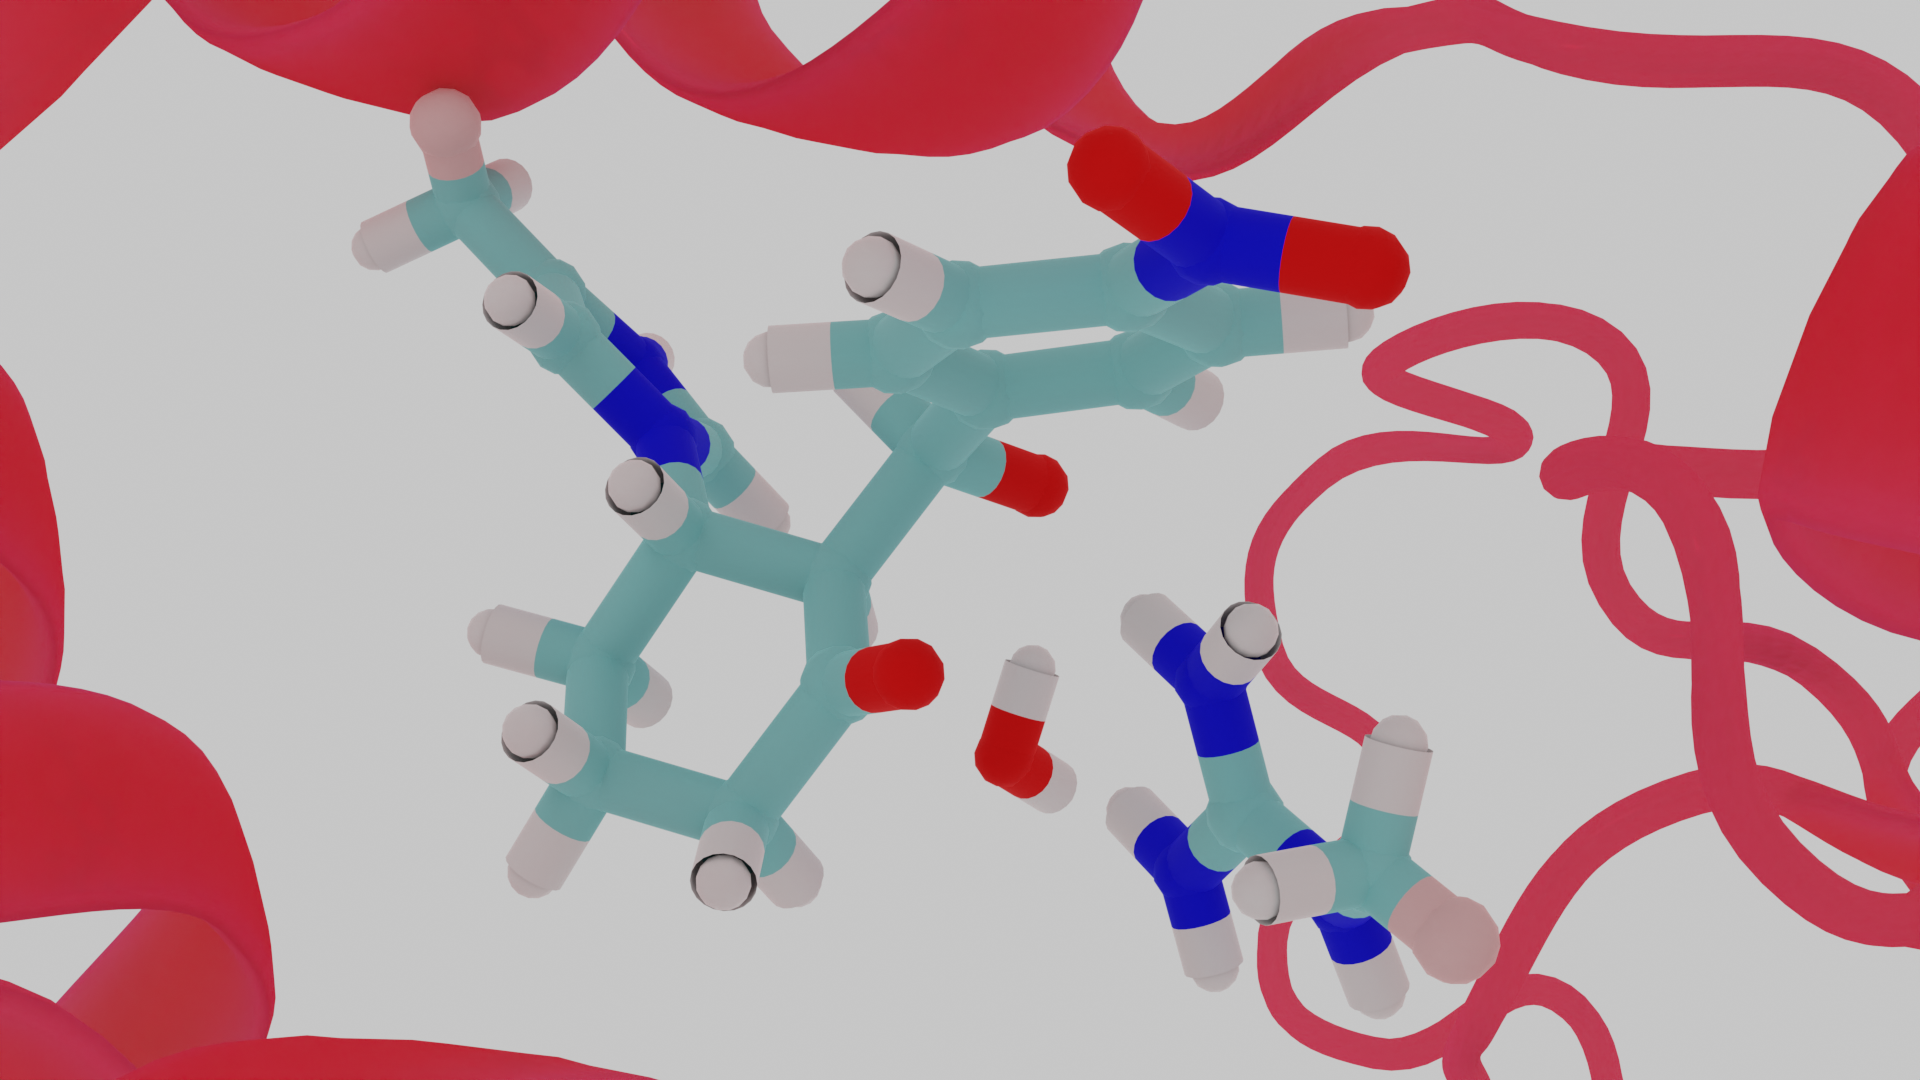
\includegraphics[scale=0.5]{figures/reac-81.png}
        
        \end{block}
        \begin{block}{yoohoo}
        
        something something
        
        \end{block}
    \end{column}
    \separatorcolumn
\begin{column}{\colwidth}
  \begin{block}{bahaha}

  \end{block}
  \begin{block}{bahaha}

  \end{block}
  \begin{block}{bahaha}

  \end{block}
\end{column}
\separatorcolumn
\begin{column}{\colwidth}
  \begin{block}{bahaha}

  \end{block}
  \begin{block}{bahaha}

  \end{block}
  \begin{block}{bahaha}

  \end{block}
\end{column}
\separatorcolumn
  \end{columns}
\end{frame}

\end{document}
